\section{202109-5 箱根山岳险天下}
	\begin{itemize}
		\item 时间限制:$5.0\texttt{ s}$.
		\item 空间限制:$512.0\texttt{ MiB}$.
	\end{itemize}
	\subsection{题目}
		\subsubsection{题目背景}
			\par ``你知道对长跑选手来说,最棒的赞美是什么吗?''
			\par ``是`快'吗?''
			\par ``不,是`强',''清濑说,``光跑得快,是没办法在长跑中脱颖而出的。天候、场地、比赛的发展、体能,还有自己的精神状态--长跑选手必须冷静分析这许多要素,即使面对再大的困难,也要坚忍不拔地突破难关。长跑选手需要的,是真正的`强'。所以我们必须把`强'当作最高的荣誉,每天不断跑下去。''
			\par 不论阿走或其他房客,全都全神贯注地聆听清濑的话。
			\par ``看了你这三个月来的表现,我越来越相信自己没看错人,''清濑接着说,``你很有天分,也很有潜力。所以呢,阿走,你一定要更相信自己,不要急着想一飞冲天。变强需要时间,也可以说它永远没有终点。长跑是值得一生投入的竞赛,有些人即使老了,仍然没有放弃慢跑或马拉松运动。''
			\par ---三浦紫苑《强风吹拂》
			\par 箱根驿传(正式名称为东京箱根间往复大学驿传竞走)是日本一项在每年 1 月 2-3 日举行的驿站接力赛,由关东学生田径联盟主办,关东的每所高校都有机会参加。在日本,箱根驿传是新年假期必看的比赛,许多家庭会一边吃年糕汤一边欣赏激烈的比赛。
			\par 今年,京都大学也想派出长跑队参加箱根驿传,田径部的长跑教练组织起一批预备役运动员,并开展了严苛的训练。
		\subsubsection{题目描述}
			\par 京都大学的训练一共会持续 $m$ 天,在训练过程中正式队员的名单可能发生变化。简单起见,我们约定在且仅在第 $t(1\leq t\leq m)$ 天结束时,会有以下三种事件之一发生:
			\begin{enumerate}
				\item 有一个学生跑 $10\texttt{ km}$ 的速度达到了正式队员要求,教练将其作为最后一名纳入正式队员的名单中,这个学生的强度为 $x$;或者速度排名在最后一位的正式队员,由于速度过慢,而被从正式队员的名单中淘汰。
					\begin{itemize}
						\item 在训练过程中,我们假定队员的速度的相对排名不会发生变化,与强度无关。
						\item 严苛的教练制订了残酷的规则:被淘汰的学生虽然依然会跟大家一起训练,但将不能再次加入本年度参加箱根驿传的正式队员的名单中。
					\end{itemize}
				\item 由于近日的训练,第 $s$ 天结束时速度排名为 $l$ 至 $r$ 的选手的强度有了变化,变为此前的 $y$ 倍。
				\item 教练在深夜想知道近日训练的效果,于是他统计了第 $s$ 天结束时速度排名为 $l$ 至 $r$ 的选手目前(即第 $t$ 天结束时)强度的和。由于这个结果可能很大,方便起见我们只考虑其模 $p$ 的值。		   
			\end{enumerate}
			\par 出于学生们的隐私考虑,事件日志有可能会被加密。
		\subsubsection{子任务}
			\par $1\leq m\leq 3\times 10^5$,$2\leq p<2^{30}$,$\text{mode}\in\{0,1\}$。
			\begin{table}[!ht]
				\centering
				\begin{tabular}{|c|c|c|}
				\hline
					测试点 & 特殊性质 & $\text{mode}$ \\ \hline
					1 & $m\leq 5000$ & 1 \\ \hline
					2 & 事件 1 中 $x>0$ & 1 \\ \hline
					3 & 没有事件 2 & 1 \\ \hline
					4 & 事件 1 中 $x$ 在 $0,1$ 中随机选取 & 0 \\ \hline
					5 & $r-l\leq 10$ & 0 \\ \hline
					6 & $r-l\leq 10$ & 1 \\ \hline
					7, 8 & 无 & 0 \\ \hline
					9, 10 & 无 & 1 \\ \hline
				\end{tabular}
			\end{table}
	\subsection{解法 A(100 分)}
		\subsubsection{原理阐释}
			\par 这个题目描述理解难度较大,我们首先解读一下题目:
			\begin{itemize}
				\item 每个人可抽象为一个节点。
				\item 排名由前到后排成一条链,那么加入操作相当于在最后加入一个节点,删除操作相当于回退一个节点。
				\item 这些节点形成了若干个有根树的集合。
				\item 若我们加多一个空的根节点,那么就变成一个有根树。
				\item 四种操作分别对应
					\begin{enumerate}
						\item 当前节点(初始为我们的空根节点)后加上一个叶子节点;
						\item 当前节点设为当前节点的父亲节点;
						\item 修改 $s$ 时对应节点的 $l,r$ 级祖先之间的链;
						\item 查询 $s$ 时对应节点的 $l,r$ 级祖先之间的链。
					\end{enumerate}
			\end{itemize}
			\par 本题出题人给了许多特殊性质,分别为:
			\begin{itemize}
				\item 离线:对应解法为树上数据结构,例如树链剖分。
				\item $x>0$:对应解法为链上数据结构,例如线段树。
				\item 没有事件 2:对应解法为无修动态数据结构,例如倍增+树上缀和。
				\item 事件 1 中 $x$ 在 $0,1$ 随机选取:对应解法为树高较矮时的统计,例如朴素求和。
				\item $r-l\leq 10$:对应解法为树上短链修改查询,例如倍增+朴素求和。
			\end{itemize}
			\par 但上述这些解法繁琐而失去一般性,下面我们根据出题人的提示,探索正确解法。
			\par 毋庸置疑,本题考察树上数据结构,且其要求为:强制在线、修改树结构、修改链、询问链。显然,我们想到的最好解决办法即为 Link-Cut Tree。
			\par 直接实现即可,时间复杂度 $\Theta(m\log m)$,空间复杂度 $\Theta(m)$。
		\subsubsection{C++ 代码实现}
			\lstinputlisting[
				style=C++,
				title={\bf 202109-5.cpp},
				tabsize=4
			]{202109-5.cpp}
		\subsubsection{提交结果}
			\begin{figure*}[htbp]
				\centering
				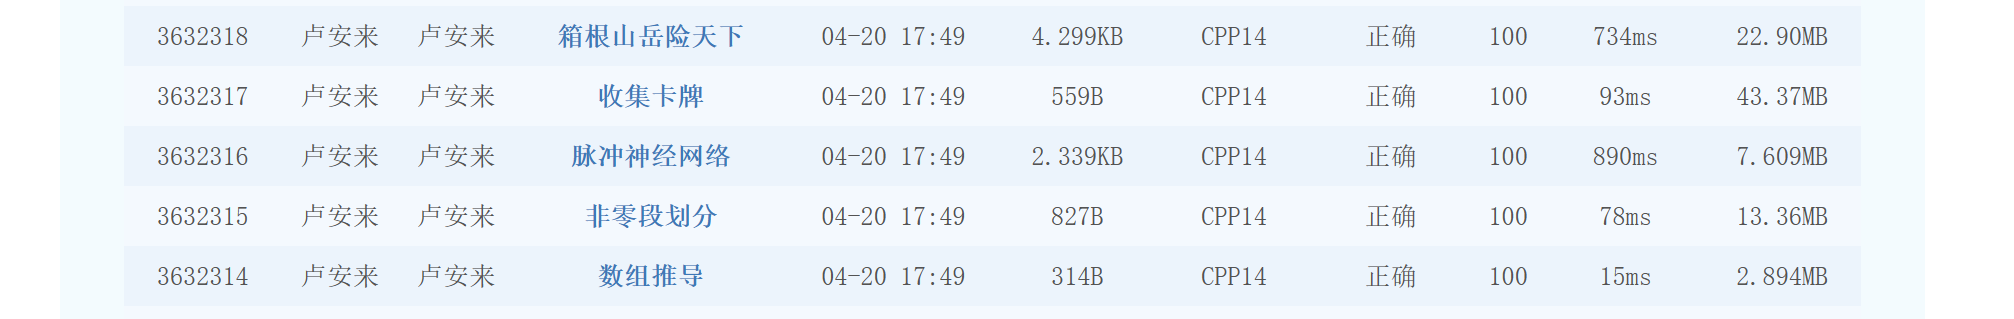
\includegraphics[width=1\textwidth]{result.png}
				\caption{提交结果}
			\end{figure*}